
\begin{figure}
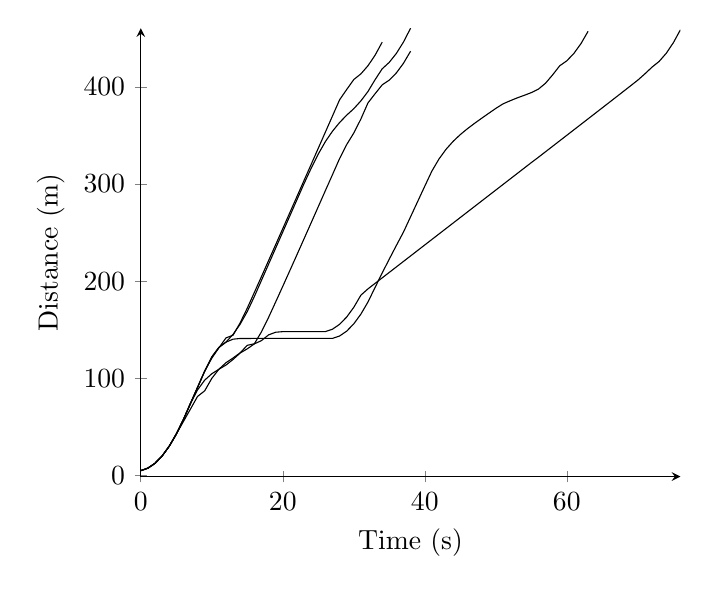
\begin{tikzpicture}
\begin{axis}[
legend style={anchor=west},
axis x line=bottom,
axis y line=left,
ymin=-1,
xlabel=Time (s),
ylabel=Distance (m),
]
\addplot[] coordinates {
(0, 5.1)
(1, 7.6)
(2, 12.6)
(3, 20.1)
(4, 30.1)
(5, 42.6)
(6, 57.6)
(7, 74.2)
(8, 90.8)
(9, 107.4)
(10, 120.738768019)
(11, 131.383856994)
(12, 141.619325226)
(13, 144.462868169)
(14, 157.236548116)
(15, 172.267552707)
(16, 188.476978399)
(17, 204.791670449)
(18, 221.182945014)
(19, 237.630080286)
(20, 254.118038366)
(21, 270.635870448)
(22, 287.175585989)
(23, 303.731343352)
(24, 320.191343352)
(25, 336.791343352)
(26, 353.391343352)
(27, 369.991343352)
(28, 386.591343352)
(29, 397.210809184)
(30, 407.440112613)
(31, 413.299229302)
(32, 421.658345991)
(33, 432.51746268)
(34, 445.876579369)
};
\addplot[] coordinates {
(0, 5.1)
(1, 7.6)
(2, 12.6)
(3, 20.1)
(4, 30.1)
(5, 42.6)
(6, 57.6)
(7, 74.2)
(8, 90.8)
(9, 107.4)
(10, 122.013587752)
(11, 131.810959273)
(12, 137.299583591)
(13, 140.338453008)
(14, 141.064129728)
(15, 141.064129728)
(16, 141.1078543)
(17, 141.1078543)
(18, 141.1078543)
(19, 141.1078543)
(20, 141.1078543)
(21, 141.1078543)
(22, 141.1078543)
(23, 141.1078543)
(24, 141.1078543)
(25, 141.1078543)
(26, 141.1078543)
(27, 141.1078543)
(28, 143.6078543)
(29, 148.6078543)
(30, 156.1078543)
(31, 166.1078543)
(32, 178.6078543)
(33, 193.6078543)
(34, 208.424832023)
(35, 222.777086793)
(36, 236.793576331)
(37, 250.570737556)
(38, 266.301785806)
(39, 282.032995562)
(40, 297.76442143)
(41, 313.289520693)
(42, 325.733629726)
(43, 335.750405982)
(44, 343.93459027)
(45, 350.822141537)
(46, 356.847263371)
(47, 362.360808729)
(48, 367.598983446)
(49, 372.701883781)
(50, 377.749031947)
(51, 382.386833584)
(52, 385.560935206)
(53, 388.547164624)
(54, 391.192857468)
(55, 394.008135518)
(56, 397.581282766)
(57, 403.654430015)
(58, 412.227577264)
(59, 421.599924932)
(60, 426.728307601)
(61, 434.356690269)
(62, 444.485072937)
(63, 457.113455606)
};
\addplot[] coordinates {
(0, 5.1)
(1, 7.6)
(2, 12.6)
(3, 20.1)
(4, 30.1)
(5, 42.6)
(6, 57.6)
(7, 74.2)
(8, 88.1937869528)
(9, 98.1587182004)
(10, 104.743292247)
(11, 109.364324297)
(12, 113.681831378)
(13, 119.481765323)
(14, 126.090075689)
(15, 130.402641712)
(16, 135.4973251)
(17, 138.864934123)
(18, 144.732543145)
(19, 147.480656214)
(20, 148.080059629)
(21, 148.109925668)
(22, 148.109925668)
(23, 148.109925668)
(24, 148.109925668)
(25, 148.109925668)
(26, 148.109925668)
(27, 150.609925668)
(28, 155.609925668)
(29, 163.109925668)
(30, 173.109925668)
(31, 185.609925668)
(32, 192.109925668)
(33, 197.756468361)
(34, 203.403018904)
(35, 209.049577888)
(36, 214.696145967)
(37, 220.342723864)
(38, 225.989312379)
(39, 231.635912404)
(40, 237.282524931)
(41, 242.929151071)
(42, 248.575792071)
(43, 254.222449335)
(44, 259.869124447)
(45, 265.515819209)
(46, 271.162535668)
(47, 276.809276171)
(48, 282.456043414)
(49, 288.10284051)
(50, 293.749671079)
(51, 299.396539348)
(52, 305.043450288)
(53, 310.690409787)
(54, 316.337424866)
(55, 321.984503973)
(56, 327.491657356)
(57, 333.138943981)
(58, 338.78715918)
(59, 344.436480066)
(60, 350.087131927)
(61, 355.739405827)
(62, 361.393684559)
(63, 367.050481962)
(64, 372.710504432)
(65, 378.374750806)
(66, 384.044681943)
(67, 389.72252457)
(68, 395.411853455)
(69, 401.118806764)
(70, 406.854931987)
(71, 413.340907499)
(72, 420.212775246)
(73, 426.065483673)
(74, 434.418192099)
(75, 445.270900526)
(76, 458.623608953)
};
\addplot[] coordinates {
(0, 5.1)
(1, 7.6)
(2, 12.6)
(3, 20.1)
(4, 30.1)
(5, 42.6)
(6, 57.6)
(7, 74.2)
(8, 90.8)
(9, 107.4)
(10, 122.013587752)
(11, 131.810959273)
(12, 137.299583591)
(13, 145.288207909)
(14, 155.776832228)
(15, 168.765456546)
(16, 184.254080864)
(17, 200.854080864)
(18, 217.454080864)
(19, 234.054080864)
(20, 250.654080864)
(21, 267.254080864)
(22, 283.854080864)
(23, 300.454080864)
(24, 316.191249359)
(25, 330.838970408)
(26, 343.623443743)
(27, 354.310609461)
(28, 363.232154784)
(29, 370.804229822)
(30, 377.452272522)
(31, 385.501604124)
(32, 395.156987246)
(33, 407.312370368)
(34, 418.49641982)
(35, 425.188266107)
(36, 434.380112393)
(37, 446.071958679)
(38, 460.263804966)
};
\addplot[] coordinates {
(0, 5.1)
(1, 7.6)
(2, 12.6)
(3, 20.1)
(4, 30.1)
(5, 42.6)
(6, 55.5397526464)
(7, 68.4860453883)
(8, 81.4425739802)
(9, 87.1664891982)
(10, 99.9664944725)
(11, 109.375173102)
(12, 116.108526495)
(13, 121.01831942)
(14, 126.322814115)
(15, 134.016196878)
(16, 135.618199019)
(17, 147.932693658)
(18, 162.747188298)
(19, 178.65123607)
(20, 194.745098012)
(21, 210.975986259)
(22, 227.306273612)
(23, 243.708913747)
(24, 260.16434969)
(25, 276.658379389)
(26, 293.180657598)
(27, 309.583631607)
(28, 326.141778452)
(29, 340.519486246)
(30, 352.434918671)
(31, 366.850351096)
(32, 383.450351096)
(33, 392.865858306)
(34, 401.983057131)
(35, 406.89741989)
(36, 414.311782648)
(37, 424.226145407)
(38, 436.640508166)
};

\end{axis}
\end{tikzpicture}
\label{tik:100:3_V, 3_V.-60, 4_S, 5_S, 5_S.-30, 6_V}
\caption{100 percent diving with GSC on route $3_V, 3_V.-60, 4_S, 5_S, 5_S.-30, 6_V$}
\end{figure}
